% Paper B manuscript for Sociological Methods & Research (anonymized for double-anonymized review).
% Author names, affiliations and acknowledgements live in title_page.tex (separate upload).
% Claim source: planning/TWO_PAPER_CLAIM_LOCK.md, Amendments C7 (2026-10-18) to C9.1 (2026-10-20), with
% planning/sprint_2026-10-11/paper-b-tier1/NUMBERS_TABLE.csv (sha256 71ee7c8c...86a4, 562 rows). The
% descriptive follow-up analyses (surface D) use the C9 rows; the C9-4 rows passed their cross-family audit
% (card t_b4030219, claim lock C9-4 append-only note of 2026-10-20): descriptive, not preregistered.
% TODO(Augusto): swap to the SMR Overleaf template at submission; this preamble follows the SMR
% format rules (12 pt, double spacing, 1.25 in margins, footnotes, author-date references).
\documentclass[12pt]{article}
\usepackage[T1]{fontenc}
\usepackage[utf8]{inputenc}
\usepackage[margin=1.25in]{geometry}
\usepackage{lmodern,microtype,amsmath,amssymb,booktabs,tabularx,array,graphicx,xcolor}
\usepackage{tikz}
\usetikzlibrary{positioning,arrows.meta}
\usepackage{setspace}
\usepackage[authoryear,round]{natbib}
\usepackage{xurl}
\usepackage[hidelinks]{hyperref}
\usepackage[labelfont=bf,font=small]{caption}
\setlength{\emergencystretch}{2em}
\widowpenalty=10000
\clubpenalty=10000
\input{macros}

\title{Synthetic Cultural Agents as Group-Level Instruments: A Preregistered Evaluation from Anchor to Respondents}
% Review copy for co-authors: compile main_review.tex (defines \showauthors). main.tex stays anonymous for SMR.
\ifdefined\showauthors
\author{Augusto Gonzalez-Bonorino$^{1,2}$ \and Kseniia Biriukova$^{2,3}$ \and Monica Capra$^{2,4}$\\[0.8em]
\small $^1$Department of Economics, Arizona State University\\
\small $^2$EconLLM Lab\\
\small $^3$Department of Information Systems, Arizona State University\\
\small $^4$Department of Economics, Claremont Graduate University}
\else
\author{}
\fi
\date{}

\begin{document}
\maketitle
\thispagestyle{empty}
\begin{abstract}
\noindent Cross-national surveys commit to items before learning whether they separate countries; language models offer a cheap first reading. The usual route simulates individuals, then averages. We ask the model only about the group. Six declared signs of country-level survey moments label synthetic preference pairs that train adapters, which read items without naming the country. On trust, they order countries as the survey does on two scenario banks. A prompt stating those signs does too, so signs carry the order. Against a retrospective criterion, a preregistered screen of held-out items gives a weak signal that registered contrasts cannot separate from questionnaire readers. Descriptively, the adapters' order does not detectably agree with respondents', and their response distributions lie farther from the survey than the base model's. That is, the instrument orders countries like a benchmark survey while answering unlike another survey's respondents. It can complement human pretesting. We have not tested pre-piloting.
\end{abstract}

\noindent\textbf{Keywords:} synthetic respondents; large language models; measurement validity; survey item screening; preregistration; cross-national measurement.

\clearpage
\doublespacing
\section{Introduction}\label{sec:introduction}

Cross-national survey programs commit to their items long before they learn how those items behave. A question about trust must be translated, pretested and fielded in many countries before a researcher sees whether its country differences follow the construct it was written for. Language models offer a cheap first reading of such items \citep{argyle2023,horton2023,buskirk2026}. A reading that flagged in advance which new items separate countries would be useful at exactly this stage. We build one such reading and check, link by link, what it does against a benchmark survey and against the respondents of a second survey.

The usual route to a synthetic reading goes through individuals. Silicon sampling describes a person in the prompt, collects the model's answer, and averages many such persons into a country figure \citep{argyle2023}. That route needs two things that are hard to supply. First, it needs a model of each simulated person. The errors of those simulated people are correlated, because one model with one set of assumptions produces all of them. Averaging more of them therefore need not cancel the bias. Second, it needs a sampling frame: someone must decide which people to simulate and in what proportions. The record so far is cautionary. Synthetic responses are sensitive to prompt wording, compress the variance of human answers and depend on the order and labelling of answer options \citep{bisbee2024,boelaert2025,wang2025,dominguezolmedo2024}. Alignment procedures change how faithfully models simulate attitudes \citep{lyman2025}, and methodological work in this journal concludes that validation against human data remains essential \citep{kozlowski2025,broska2025}. Most empirical work asks whether a model reproduces answers that people already gave, whether it is prompted \citep{santurkar2023,durmus2024} or fine-tuned on survey response distributions \citep{cao2025,suh2025}. In the fine-tuned case the human survey sits inside the training signal. Language-model pretesting has also been studied as flaw detection in question wording \citep{sturgis2026}. Whether a method can say which new items will separate countries in an intended direction is a different test. It needs a decision rule fixed before the human criterion is read.

We take a route that never models individuals. Cross-national research usually wants a country-level quantity, such as how countries rank on generalized trust. A probability survey such as the Global Preferences Survey \citep[GPS;][]{falk2018} has already aggregated people into such quantities, with sampling weights. We take its country-level moments as declared inputs and ask the model only for a group-level reading of new item text. In other words, the survey aggregates people, and the language model reads items at the level of the group. An order of countries can survive this design without a representative respondent. It requires only that the instrument's score rise with the group's latent preference. The design has a price. A single choice policy per country has no spread within the country built in, so it can carry an order and has no reason to match the distribution of respondents' answers. This is the representative-agent problem \citep{kirman1992}, and it gives a reason to expect that order and distribution can come apart. Because country-level agreement says nothing about individuals \citep{robinson1950}, we chose the country as the unit and keep our claims there.

Modelling the group directly is not new on its own. SubPOP \citep{suh2025} and Group Preference Optimization \citep{zhao2023gpo} predict group-level responses without simulating individuals, but they train on human response distributions and name the group. What is specific here is the combination of three features, and each is a choice a researcher can inspect. First, the inputs are declared aggregate moments. The researcher states which six GPS moments enter, and a sign rule turns them into labels, so nothing about the conditioning hides in a country name or in human answers. Second, the training data are synthetic preference pairs. Each country's sign profile labels one shared bank of generated response pairs. Direct Preference Optimization \citep{rafailov2023}, which we read as a regularized Bradley--Terry pairwise choice model, then fits one adapter per profile. No human survey answer enters training. Therefore, a human survey is a criterion the method has never seen, which is not true of models fitted to response distributions. Third, the group is unnamed at evaluation. Items are scored with prompts that never mention a country, so whatever the adapters carry comes from the conditioning. A country-token channel is closed by construction.

We evaluate the construction along a chain of three links, treating each as a separate measurement question in the way \citet{wallach2025} propose for generative systems. The anchor is the GPS, the instrument is the set of adapters, and the respondents are the people who answered Wave~7 of the World Values Survey (WVS). Prompted models have been compared with the GPS across countries and found to be weak proxies for it \citep{chen2026}. We built the construction on a purposive development panel of \dc{16}{dev_countries} countries. We then evaluate it on all \dc{42}{countries} countries covered by both the GPS and Wave~7, with a second set of adapters for all \dc{64}{cells} sign profiles on a newly generated scenario bank. At the first link we ask whether training installs the synthetic labels, whether the order of countries survives the new bank, and whether a prompt does as well. A factorial over the \dc{64}{cells} sign profiles asks whether the six declared dimensions behave as separate inputs. At the second link we ran a preregistered screen of \dc{223}{pool_items} Wave~7 items that no adapter was built for. A probe that reads only the adapters' scores assigns each item a dimension and a direction, and a fixed rule selects the strongest assignments before any human value is read. That criterion is retrospective, because the survey existed before the probe. Finally, descriptive analyses added after the registered results had been read set the adapters beside the respondents' composites and response distributions.

What we found on the first link is an order of countries that the declared signs carry. Training installs each country's synthetic labels on scenarios the adapters never saw. On trust, the adapters keep the GPS order of countries when the scenario bank is replaced, whereas a prompt that names the country does not. A prompt that states the same six signs keeps the trust order as well, and the contrast between the adapters and that prompt is unresolved. That is, the signs carry the order, and the evidence gives the trained weights no separate credit. The order is specific to trust. Each declared sign moves its own surface in the intended direction and also moves the others, often by more. Trust is the one surface where its own sign dominates.

Checked against people, the instrument answers unlike them. The retrospective screen gives a weak signal. The registered null is rejected, yet the signal is a small fraction of what two human survey waves achieve on the same items, and its country-bootstrap interval reaches zero. Registered contrasts do not distinguish the adapters from careful readers of the questionnaire on the few items they share, and no dimension passes both the second-bank check and the screen. Descriptively, the adapters' order of countries does not detectably agree with the respondents' composite on any surface. Notably, the GPS's own agreement with those respondents is loose. On response distributions the ranking reverses. The adapters sit farther from the survey's response distributions than the base model does, whereas a country-named prompt sits closer and has no trust order. The separation of order from distributional fidelity is known \citep{dasilva2026,wangc2026}. What this case adds is one method, on one anchor, that answers the two questions in opposite directions. Put plainly, a model asked only about the group can order countries the way a cross-national survey does while answering unlike the people in them.

Our contributions are two.
\begin{enumerate}
\item \textbf{An inspectable group-level conditioning method.} Declared aggregate moments, synthetic preference pairs and an unnamed group at evaluation define a construction whose information budget is on the record. A reader can see what the method was given and check where its readings depart from people.
\item \textbf{A reusable evaluation protocol.} We separate the three links and state what a favorable or unfavorable result at each permits. The protocol includes a screen of new items whose probe is fixed before any human value is read, and a permutation null that absorbs the probe's selection rate. It adds a human ceiling from two survey waves, item-matched comparators that read only the questionnaire, and a factorial that tests whether declared dimensions stay separate.
\end{enumerate}

What the paper shows is bounded by its design: one anchor, one instrument family and one base model. We do not show that trained weights improve on a prompt that states the same signs. Nor do we show that the adapters agree with respondents beyond the weak retrospective signal, or that screening would change which items a researcher fields. Pre-piloting is a prospective use that remains untested. The instrument carries no information about magnitudes or about variation among people within a country, and its readings concern differences among countries. Within these bounds a survey designer can consult it beside human pretesting as a complement, never in its place.

Section~\ref{sec:background} places the method among current uses of synthetic respondents and in the measurement literature on cross-national comparability. Sections~\ref{sec:instrument} and~\ref{sec:design} describe the construction and the design with its registration, Section~\ref{sec:results} reports the results, and Section~\ref{sec:discussion} discusses what they permit.

\section{Synthetic Respondents as Measurement Instruments}\label{sec:background}

\paragraph{Synthetic respondents and the criterion they need.} A language model conditioned on a description of a population can be asked to stand in for a sample of its members. In silicon sampling the description enters the prompt and the model's answer distribution is read as an estimate of the population's \citep{argyle2023}; in the homo silicus program the model plays an economic agent in a stylized decision problem \citep{horton2023}; a systematic review maps how fast these uses have spread across survey research \citep{buskirk2026}. Fine-tuning on survey responses is one response to the evidence on prompted models \citep{suh2025,cao2025,krsteski2026}. Two reviews in this journal draw the conclusion that matters here: validation against human data remains essential \citep{kozlowski2025}, and model predictions are best treated as potentially informative observations while human subjects remain the gold standard \citep{broska2025}. Both require a criterion against which the synthetic reading can fail. Our evaluation supplies one criterion for each link of the chain.

\paragraph{Construct, measure, and anchor.} Three objects have to be kept apart. A construct is a theoretical preference attribute, such as generalized trust. A measure operationalizes it through observed answers, such as the response distribution to a WVS question about whether most people can be trusted. An anchor is an aggregate score that conditions the instrument, such as a country's GPS trust coordinate. The GPS supplies anchors for six economic preferences (trust, risk taking, patience, altruism, positive reciprocity and negative reciprocity), measured with experimentally validated modules in a common design across countries \citep{falk2018}. We treat these coordinates as declared aggregate moments: the researcher chooses them, and nothing in the construction certifies them as the right moments for a given survey. Mapping a WVS item to a GPS dimension makes the item a candidate indicator, and an average of such items a proposed composite. Agreement between instrument and anchor, between instrument and people, and between anchor and people are three different facts, and they are the three comparisons that the chain makes. The multitrait--multimethod logic of \citet{campbellfiske1959} applies directly: the human survey is the other method, and an instrument that agrees with its own anchor has passed a construction check without yet meeting a criterion.

\paragraph{Cross-national comparability.} The unit of analysis is the country. Country-level agreement does not establish that an item measures the same construct for individuals in different countries, because loadings and intercepts can differ across groups in ways that leave country means comparable for some purposes and misleading for others \citep{steenkamp1998,davidov2014}. Work in this journal argues that country-level composites can suffice for simple group comparisons despite noninvariance while understating uncertainty \citep{bratt2025}, and that unaddressed measurement error and, less so, noninvariance bias multilevel estimates \citep{pokropek2025}. Every comparison with respondents below concerns country rankings, with no claim about invariance or individual-level validity.

\paragraph{What is left open.} Prior evaluations score models on questions whose human answers are known, or fine-tune them on human survey responses. What remains open is, link by link, what an instrument built from declared aggregate inputs alone preserves of its anchor and of the respondents' answers, with the selection rule for new items registered before the human criterion is read.

\section{The Instrument}\label{sec:instrument}

The instrument is the middle link of the chain. It maps declared aggregate preference signs from the anchor into choice policies and reads them on survey items without naming any country. A language model is treated throughout as a conditional distribution over response sequences given a prompt \citep{ludwig2026}.

\subsection{From declared signs to a shared pair bank}

Every input to the instrument should be declared and inspectable. Let $z_c=(z_{c1},\ldots,z_{cK})$ be the GPS coordinates of country $c$ on the $K$ dimensions of trust, risk taking, patience, altruism, positive reciprocity and negative reciprocity. Only the sign profile $s_c$, with $s_{ck}=1\{z_{ck}\geq 0\}$, enters the construction. A teacher model and a response generator produce a shared bank of scenarios, each with two responses intended to express a higher and a lower level of one dimension $k_i$. For country $c$, the chosen and rejected responses on pair $i$ are
\begin{equation}
(y_{w,ci},\,y_{\ell,ci})=\begin{cases}(y_i^{+},\,y_i^{-}), & s_{c,k_i}=1,\\ (y_i^{-},\,y_i^{+}), & s_{c,k_i}=0.\end{cases}
\label{eq:sign_rule}
\end{equation}
The scenario and response text is identical for every country. Only the label changes. No scenario names a country or reuses WVS question wording. The intended loading of each pair is a generator judgment and has not been verified as a trait manipulation. Two countries with the same sign profile receive identical labels, so the instrument cannot distinguish them, and nothing in the construction carries the magnitude $|z_{ck}|$. That is the information budget: six bits per country.

\subsection{Preference optimization as regularized pairwise choice}

Labeled pairs are choice data, so we fit each sign profile with a pairwise choice model, Direct Preference Optimization. Under the Bradley--Terry model, the probability that $y_w$ is chosen over $y_\ell$ after prompt $x$ is $\sigma\{r(x,y_w)-r(x,y_\ell)\}$, with $\sigma$ the logistic function and $r$ a latent utility index. This is the binary logit of random-utility theory \citep{bradleyterry1952}. DPO writes the index as $r(x,y)=\beta\log\{\pi_\theta(y\mid x)/\pi_{\mathrm{ref}}(y\mid x)\}$ up to a prompt-specific constant that cancels from pairwise differences. It then minimizes the negative log likelihood of the labeled pairs,
\begin{equation}
\mathcal{L}_c(\theta)=-\frac{1}{|\mathcal{D}_c|}\sum_{(x,y_w,y_\ell)\in\mathcal{D}_c}\log\sigma\!\left\{\beta\log\frac{\pi_\theta(y_w\mid x)}{\pi_{\mathrm{ref}}(y_w\mid x)}-\beta\log\frac{\pi_\theta(y_\ell\mid x)}{\pi_{\mathrm{ref}}(y_\ell\mid x)}\right\}.
\label{eq:dpo}
\end{equation}
The parameter $\beta$ penalizes departures from the reference policy, which makes the estimator a regularized Bradley--Terry fit \citep{rafailov2023}. Because the labels are deterministic, the likelihood is a fitting criterion and says nothing about noise in human choices. Each adapter is a low-rank update to a quantized Llama~3.1 8B Instruct base model \citep{hu2022,dettmers2023}, trained jointly on all six dimensions for one epoch on \dc{526}{train_rows} of the \dc{658}{bank_pairs} pairs, with LoRA rank \dc{16}{lora_r} and $\beta=\dc{0.1}{dpo_beta}$. A joint adapter does not isolate any single dimension. Whether the dimensions separate in practice is the subject of the factorial in Section~\ref{sec:design}.

\subsection{Two cohorts and two prompt routes}

Two kinds of question need two sets of adapters: how countries compare and how each sign acts. The first cohort has one adapter for each of the \dc{42}{countries} countries in the intersection of the GPS and WVS Wave~7, trained on the original scenario bank. These countries realize \dc{26}{profiles_realized} distinct sign profiles. The second cohort is trained on a second, independently generated bank of \dc{658}{bank_pairs} pairs under the same sign rule and text restrictions. It contains one adapter for each of the \dc{64}{cells} possible sign profiles, a full $2^6$ factorial in the six sign bits. The labels depend on the country only through its sign profile. Therefore, each country takes its profile's adapter in country-level comparisons. Most of the \dc{64}{cells} profiles are design cells that no country realizes.

Adapters are one channel for the signs, so we also score two prompt routes. The sign-profile prompt route gives the base model the same six signs in words, with no country name and no adapter. It carries the same declared information through a different channel and is the natural comparison for the trained route. The country-named persona route replaces the neutral opening of the evaluation prompt with ``Answer this questionnaire as a typical adult living in'' followed by the country's name, and supplies no signs. It changes the information as well as the channel, because the model can draw on whatever it associates with the country name. Naming the population is the comparison a survey researcher would reach first, so we score it on all \dc{42}{countries} countries.

\subsection{Readout}

Each item needs one number, so we turn the model's code probabilities into a score. For an item $q$ with candidate response codes $j$, the instrument computes the teacher-forced log probability of each code after the rendered item prompt and normalizes over the supplied codes,
\begin{equation}
\widehat P_u(j\mid q)=\frac{\exp \ell_{uqj}}{\sum_h \exp \ell_{uqh}},
\qquad
y_{uq}=\sum_j g_q(j)\,\widehat P_u(j\mid q),
\label{eq:readout}
\end{equation}
where $\ell_{uqj}$ is the summed token log probability of code $j$ for unit $u$ (an adapter or a prompted profile) and $g_q$ is the item's recode. That is, the score $y_{uq}$ is the expected recoded response. Apart from the persona route, no evaluation prompt names a country. The prompt template, option order and recode are frozen in a scoring specification whose hash every run must reproduce before a model is loaded. On the original \dc{23}{strict_items}-item WVS battery, we average item scores into seven surfaces. Five follow trust, risk taking, altruism and the two reciprocities. Patience contributes two surfaces, one for each of its two items. We call this the strict battery. The normalized code probabilities are a scoring convention, and their dispersion need not match any human population's response distributions.

\section{Evaluation Design}\label{sec:design}

The evaluation follows the chain, and each comparison permits one kind of statement. A construction check asks whether the adapters encode what they were trained on (anchor to instrument). A second-bank check asks whether the anchor's order survives a change of scenario text. A factorial asks whether the declared dimensions behave as separate inputs. A held-out screen asks whether the instrument's readings of new items agree with an existing human survey (instrument to respondents). Descriptive analyses added after the registered results had been read place the instrument beside the respondents and beside its own labels. Every statistic carries the label of the surface it was computed on (Table~\ref{tab:surfaces}), and statistics from different surfaces are never pooled.

\begin{table}[htbp]
\centering
\caption{Evaluation surfaces. Every statistic belongs to one, and the status column says how its analysis was fixed.}\label{tab:surfaces}
\small
\renewcommand{\arraystretch}{1.15}
\begin{tabularx}{\textwidth}{@{}l>{\raggedright\arraybackslash}X>{\raggedright\arraybackslash}p{0.27\textwidth}@{}}
\toprule
Label & Units, items and comparison & Status \\
\midrule
S1 & First-cohort country adapters, strict battery: adapter--GPS rank correlation (model side only) & Basis of the second-bank rule \\
S2 & Second-cohort profile adapters: same statistic as S1 & Rule fixed before training \\
H & Second-cohort adapters on held-out Wave~7 items: signed agreement of selected items with human country means & Preregistered; retrospective criterion \\
F & Second-cohort adapters and prompted profiles: main effects of six sign bits on seven surfaces (model side only) & V5 planned; rest exploratory \\
R, N & One unseeded retrain; two near-zero refits (model side only) & Predeclared checks \\
P & Country-named prompt on the base model: persona--GPS rank correlation (model side only) & One contrast planned; rest descriptive \\
D & Adapters, factorial and prompt routes: agreement with the GPS and the Wave~7 composite, distance to survey distributions, decomposition of main effects, label recovery & Descriptive, not preregistered \\
\bottomrule
\end{tabularx}
\end{table}

\subsection{Second-bank check}\label{sec:design-bank}

For each surface of the strict battery we compute the Spearman correlation between the adapters' surface composites and the GPS coordinate of the surface's own dimension over the \dc{42}{countries} countries, first for the first cohort (S1) and then for the second cohort with each country assigned its profile's adapter (S2). Intervals come from a profile-block bootstrap that resamples the \dc{26}{profiles_realized} realized sign profiles, with \dc{2,000}{boot_draws} draws, seed \dc{20261011}{seed_c3}, and percentile limits. The imprint set is the \dc{4}{imprint_dims} dimensions whose first-cohort interval excluded zero: trust, risk taking, positive reciprocity and altruism; patience and negative reciprocity were flat and are reported without interpretation. The rule was fixed before the second cohort was trained: for an imprint dimension whose second-bank interval includes zero, no sentence about carry-over to the second bank is written. We also report the agreement between the two banks over the \dc{26}{profiles_realized} shared profiles; it measures how much the scenario text changes the instrument and involves no human data.

\subsection{The country-named prompt}\label{sec:design-persona}

The persona route was scored on the strict battery for each of the \dc{42}{countries} countries in one run on the frozen stack. We compute the persona--GPS correlation for each surface (P) and one planned contrast, fixed in a design note committed before any persona was scored: the first cohort's trust correlation minus the persona route's, recomputed on every draw of the profile-block bootstrap above. All other differences are descriptive.

\subsection{The held-out screen}\label{sec:design-screen}

\paragraph{Item pool.} The pool was built from WVS Wave~7 metadata alone: ordinal questions with two to eleven contiguous response codes outside the battery used to develop the adapters. A text review excluded items with non-monotone codes or factual content and repaired wording that did not extract, which leaves \dc{223}{pool_items} items that no adapter was built for (online supplement).

\paragraph{Probe.} All \dc{64}{cells} second-cohort adapters scored every pool item under the frozen specification. For each item $i$, the probe regresses the \dc{64}{cells} adapter scores on an intercept, the six sign bits coded $\pm\dc{0.5}{x_code}$, and their \dc{15}{interactions} two-way interactions, which leaves \dc{42}{error_df} error degrees of freedom. With $t_{d}$ the main-effect $t$ statistic of dimension $d$, the item's assigned dimension is $d_i=\arg\max_d|t_d|$, or none when the largest $|t_d|$ is below \dc{2.0}{t_threshold}, and its sign is $s_i=\operatorname{sign}(b_{d_i})$. The primary rule keeps items whose assigned dimension is in the imprint set and whose $|t|$ is at least \dc{2}{t_threshold}, up to the top \dc{25}{top_share} percent of all pool items by $|t|$, which caps the selection at \dc{56}{max_selected} items. The secondary rule keeps every imprint item above the threshold and is a reliability check only. The probe reads model scores only; the permutation null absorbs the rate at which noise items cross the threshold.

\paragraph{Statistic and criterion.} For each selected item, the signed item agreement is
\begin{equation}
a_i = s_i\cdot\rho\big(\bar h_{ci},\,z_{c,d_i}\big),
\qquad
A=\frac{1}{|S|}\sum_{i\in S}a_i,
\label{eq:screen}
\end{equation}
where $\rho$ is the Spearman correlation over the \dc{42}{countries} countries, $\bar h_{ci}$ is the survey-weighted Wave~7 mean of item $i$ in country $c$ with negative codes set to missing, and $S$ is the selected set. An item--country cell that was never fielded enters as missing and is not imputed. $A$ is the mean signed agreement with human country differences: it is positive when those differences run in the direction the instrument assigned, against the GPS coordinate of the assigned dimension.

\paragraph{Inference.} The registered test is a permutation null over items: draw as many items as were selected from the pool, give them the selected items' dimension and sign pairs in random order, and recompute $A$; \dc{10,000}{perm_draws} draws, seed \dc{20261015}{seed_screen}, one-sided $p$ equal to the share of null draws at or above the observed $A$. A \dc{95}{ci_level} percent interval for $A$ comes from \dc{2,000}{boot_draws} bootstrap resamples of the \dc{42}{countries} countries. The readings were fixed in advance: if $A$ is not above the null at one-sided $\alpha=\dc{0.05}{alpha}$, the adapters do not screen better than random assignment; if $A$ is above the null but below one third of the human ceiling, a screening signal exists but is weak.

\paragraph{Human ceiling.} For each selected item fielded in both WVS waves 6 and 7 we correlate the two waves' country means over the \dc{28}{ceiling_countries} countries with both waves \citep{wvsts2022} and average over items, which gives the agreement two human surveys reach on these items; the ratio of $A$ to it is a benchmark only.

\paragraph{Per-dimension readings.} The registered analysis also reports $A_d$, the mean of $a_i$ over the selected items assigned to dimension $d$, with an interval from the same country resamples. These intervals are unadjusted, so we add exploratory Bonferroni intervals for the four imprint dimensions from the same draws at the \dc{98.75}{bonf_level} percent level.

\paragraph{Comparators.} Two comparators read only the questionnaire and saw no model score or human response: a face-valid rule that assigns an item to the one dimension whose construct words its wording contains, and a typed decision model (jev-1.13.0) run \dc{5}{jev_runs} times, which assigns an item when at least \dc{3}{jev_majority} runs agree on dimension and sign (online supplement). The registered primary contrast is coverage-matched, $D_{\mathrm{common}}=A_{\mathrm{adapter}}-A_{\mathrm{comparator}}$ on the items both assign, with an interval from the paired country bootstrap. An interval above zero would mean the adapters find structure the wording does not reveal; one that covers zero was registered as ``the adapters match a careful reader''; one below zero would favor the reader. The contrast on each route's own items is reported beside it, and the preregistration named in advance that both comparators concentrate on trust.

\paragraph{Readout variants and the prompt route.} The probe was re-estimated on three re-scorings of the pool (options reversed, two prompt paraphrases), and the selection was declared dependent on wording if more than half of the selected items changed dimension or sign. The same probe and test were applied to the \dc{64}{cells} prompted profiles.

\subsection{Registration, blinding and amendments}\label{sec:design-prereg}

The screen was registered in a document committed to the project repository and timestamped by a pushed git tag before any held-out item was scored by an adapter, when no selection existed and no held-out human value had been read. A freeze guard enforced the order of work (a timeline is in the online supplement): score the held-out items, run the probe, freeze the hashes of the selection and the item pool, and only then join the human data.

Two amendments were made, both before any human held-out value was read. Amendment~1 repaired \dc{12}{repaired_items} items whose standalone wording could not be answered as written, under the pool rule and override mechanism already registered, and every route was re-scored as one run. We disclose that the first probe pass had been computed and read before the repairs were chosen, and that two repaired items (Q153 and Q157) were in its top quartile. The comparators had assigned the pool on the pre-repair wording, so Amendment~2 removed the repaired items from both comparator routes before any comparator statistic was computed; it affected one item (Q82), not in the adapter selection. That decision preceded any human value; the amendment text, written after the primary statistic was read, records it.

The criterion is retrospective. The Wave~7 file is public, existed before the probe, the pool and the adapters, and is the only human source in this study. Registration guards against tuning the probe to the criterion; it cannot make the criterion prospective, so results on surface H are labelled retrospective throughout. The online supplement discloses the provenance gaps, none of which touches a statistic reported here.

\subsection{The sign-profile factorial}\label{sec:design-factorial}

The second cohort covers all \dc{64}{cells} sign profiles, so the strict-battery composites form a full factorial in six binary factors. For each of the seven surfaces we fit the probe's regression. A main effect is the difference between the mean composites of profiles with the bit set and without it. Because the bits were assigned by design, this is a causal statement about the instrument and carries no implication about how preferences operate in people. Each bit has an own surface (patience owns two). The analysis plan set one acceptance check, separate from the held-out registration: at least \dc{4}{v5_required} of the six bits must move their own surface more than any other (V5), against a binomial reference with a one-in-seven chance of a hit. Exploratory views divide effects by each surface's standard deviation over the \dc{64}{cells} profiles, count the surfaces whose largest mover is their own bit, and report the first principal component's variance share and the mean absolute correlation between surfaces. The same analyses on the \dc{64}{cells} prompted profiles contrast two instruments that carry the same declared information.

\subsection{Retraining noise and the near-zero margin}\label{sec:design-noise}

One profile adapter was retrained without a fixed seed, which gives a noise floor for the pipeline. A predeclared sensitivity check also removes the training pairs of every dimension whose GPS coordinate lies within \dc{0.10}{near_zero_cut} of zero and refits two countries (Great Britain and Colombia), each beside a size-matched control; the rule was to report the margin and never to promote it.

\subsection{Descriptive follow-up analyses}\label{sec:design-desc}

Four further analyses were added after the registered results had been read: three columns of agreement, distance to the survey distributions, a decomposition of the factorial's cross effects, and held-out label recovery. The last two are defined with their results. None is preregistered or tests a rule fixed in advance; we label their numbers D and read them as descriptions. Their human input is the Wave~7 file used for the screen, so every comparison with respondents is retrospective.

\paragraph{Three columns.} For each of the seven surfaces we compute three Spearman correlations over countries: the adapter composite with the GPS coordinate of the surface's own dimension, the adapter composite with the Wave~7 composite of the same items, and that human composite with the GPS. The adapter columns use the first-cohort adapters (the second cohort is in the supplement) with the profile-block bootstrap above, and the human--GPS interval resamples countries (seed \dc{20260905}{seed_country}). The human columns of risk taking cover one country fewer, which has no valid answer to the risk item.

\paragraph{Distance to the survey distributions.} For country $c$ and item $q$, the total variation distance between the model's option probabilities and the survey-weighted human answer shares is
\begin{equation*}
\mathrm{TVD}_{cq}=\tfrac{1}{2}\sum_j \bigl|\widehat{P}_c(j\mid x_q)-P^{H}_c(j\mid q)\bigr|,
\end{equation*}
where $j$ runs over the answer codes and $P^{H}_c$ is the share of valid human answers equal to $j$. The headline statistic is the mean over items within a country and then over countries. We score four cells on the same frozen stack: the base model, the first-cohort adapters, the country-named persona prompt on the base model, and the adapters with the persona prompt together (gates in the supplement). Contrasts are paired differences of country means, each with a profile-block and a country interval (\dc{2,000}{boot_draws} draws each). The interaction contrast is the adapters' effect with the persona prompt minus their effect without it; zero means the two add. The human answer shares enter the distances and are not reported.

\section{Results}\label{sec:results}

We report the results along the chain, and each statistic belongs to one surface of Table~\ref{tab:surfaces}. Everything computed against the Wave~7 file is retrospective. Exact values are in the text, Table~\ref{tab:checks} and the online supplement.

\subsection{Anchor to instrument: what training installs}\label{sec:res-recovery}

Every training pair of a country carries a label. The chosen completion is the one that goes with the sign of the country's GPS coordinate on the pair's own dimension. The first question is whether that installation carries over to pairs the adapters never saw. This is a construction check on the synthetic labels (descriptive, no human data). We split the training pairs once into a training part and a held-out part that the adapters never saw. Recovery is the share of held-out pairs on which the adapter favors the chosen completion more than the base model does, and accuracy is the share on which it prefers that completion outright. Definitions and gates are in the online supplement.

Recovery is \cl{0.940}{C9_label_recovery_recovery_profile_block} \ci{0.926}{0.952}{C9_label_recovery_recovery_profile_block} and accuracy is \cl{0.816}{C9_label_recovery_accuracy_profile_block} \ci{0.771}{0.856}{C9_label_recovery_accuracy_profile_block}. The base model's accuracy is \cl{0.489}{C9_label_recovery_base_accuracy_profile_block} \ci{0.471}{0.506}{C9_label_recovery_base_accuracy_profile_block}. That interval includes one half, so the base model shows no detectable preference for the chosen completions before training. The mean margin shift is \cl{40.3}{C9_label_recovery_mean_margin_shift_profile_block} \ci{28.2}{54.1}{C9_label_recovery_mean_margin_shift_profile_block} nats. Training installs each country's synthetic labels on scenarios the adapter never saw, which is construction fidelity. It says nothing about whether the labels order countries like the GPS, and nothing about respondents. Notably, the distance results below show that the same adapters lie farther from the survey's response distributions than the base model does.

\subsection{Anchor to instrument: the trust order and what carries it}\label{sec:res-bank}

The first cohort encodes four of the six declared signs on the strict battery (S1). Over the \dc{42}{countries} countries, the adapter--GPS Spearman correlation is \cl{0.744}{B2_cohort1_trust_rho} \ci{0.500}{0.865}{B2_cohort1_trust_rho} for trust and \cl{0.435}{B2_cohort1_risktaking_rho} \ci{0.085}{0.686}{B2_cohort1_risktaking_rho} for risk taking. It is \cl{0.488}{B2_cohort1_posrecip_rho} \ci{0.120}{0.695}{B2_cohort1_posrecip_rho} for positive reciprocity and \cl{0.406}{B2_cohort1_altruism_rho} \ci{0.020}{0.676}{B2_cohort1_altruism_rho} for altruism. These four form the imprint set that the screen later uses.

The second cohort tests whether the order survives a change of scenario text (S2). Trust keeps its agreement with the GPS, at \cl{0.803}{B2_bank2_trust_rho} \ci{0.615}{0.876}{B2_bank2_trust_rho}. The other three imprint dimensions keep positive point estimates, but their intervals now include zero (Table~\ref{tab:checks}). Therefore, \cl{1}{B2_n_imprint_kept} of the \cl{4}{B2_n_imprint_kept:n} imprint dimensions passes the second-bank check and \cl{3}{B2_n_imprint_dropped} do not. Under the rule fixed before the second cohort was trained, we write no sentence about the other three carrying over. Trust is the dimension on which retention of the anchor's order is replicated across scenario banks. The banks also agree profile by profile. Over the \dc{26}{profiles_realized} shared profiles, the rank correlation between first-bank and second-bank trust composites is \cl{0.907}{B2_bank_to_bank_trust_spearman} \ci{0.774}{0.957}{B2_bank_to_bank_trust_spearman}. Risk taking is the least stable surface, at \cl{0.544}{B2_bank_to_bank_risktaking_spearman} \ci{0.187}{0.772}{B2_bank_to_bank_risktaking_spearman}, which fits its loss on the second bank (the online supplement gives every surface). This agreement measures how much the scenario text changes the instrument and says nothing about people.

What carries the trust order? The comparison a survey researcher would reach for first is a prompt that names the population. It does not reproduce the order (P): the persona--GPS correlation over the \dc{42}{countries} countries is \cl{0.028}{PX_persona_trust_rho} \ci{-0.339}{0.381}{PX_persona_trust_rho}. The planned contrast with the first cohort is \cl{0.716}{PX_D_cohort1_trust} \ci{0.191}{1.154}{PX_D_cohort1_trust}, and the reading is the same under a country bootstrap. A prompt that states the same six signs in words, with no adapter and no country name, tracks trust as closely as the adapters do. It reaches \cl{0.773}{PX_signprompt_trust_rho} \ci{0.584}{0.844}{PX_signprompt_trust_rho} (panel A of Figure~\ref{fig:route}, which sets all routes side by side). That is, on trust what separates the routes is whether the declared sign is supplied, whichever channel carries it. The contrast sets declared signs against a country name and says nothing about trained weights against prompting. On the other surfaces the persona route's intervals include zero, except for patience, which it orders positively on one item and negatively on the other (online supplement).

\subsection{Inside the instrument: the sign-profile factorial}\label{sec:res-factorial}

The factorial asks whether the six declared signs behave as separate inputs (F). On the trained route, every sign bit moves its own surface in the intended direction (panel A of Figure~\ref{fig:factorial}; the online supplement gives each effect with its $t$ statistic). All seven own effects are positive, from \cl{0.364}{FX_adapter64_trust_own_beta} for trust ($t=\cl{16.74}{FX_adapter64_trust_own_t}$) to \cl{0.124}{FX_adapter64_posrecip_own_beta} for positive reciprocity ($t=\cl{3.02}{FX_adapter64_posrecip_own_t}$), and \cl{0}{FX_adapter64_own_effects_wrong_signed} of \cl{7}{FX_adapter64_own_effects_wrong_signed:n} point the wrong way.

The planned separability check fails. Only \cl{2}{FX_adapter64_V5_hits} of the \cl{6}{FX_adapter64_V5_hits:n} bits move their own surface more than any other surface, where at least \dc{4}{v5_required} were required (binomial $p=\cl{0.207}{FX_adapter64_V5_p_binomial}$). They are the bits for altruism and negative reciprocity. Scale-free views agree (online supplement). Each bit moves its own surface and also moves others, often by more. The risk-taking bit moves the altruism surface by \cl{0.983}{FX_adapter64_risktaking_bit_on_altruism}, against the altruism bit's own effect of \cl{0.242}{FX_adapter64_altruism_own_beta}. The trust bit is the largest mover on \cl{3}{FX_adapter64_surfaces_largest_mover_is_trust_bit} of the \cl{7}{FX_adapter64_surfaces_largest_mover_is_trust_bit:n} surfaces. One common direction carries \cl{51.3}{FX_adapter64_pc1_share:pct}\% of the variance of the seven standardized surfaces, and the mean absolute correlation between surfaces is \cl{0.395}{FX_adapter64_mean_abs_inter_surface_r}. In other words, each sign keeps its intended direction on its own surface, while the size of its effects spreads across the others.

The prompted route fails the check by the same count, \cl{2}{FX_signprompt64_V5_hits} of \cl{6}{FX_signprompt64_V5_hits:n} (binomial $p=\cl{0.207}{FX_signprompt64_V5_p_binomial}$), so V5 does not separate the routes. What separates them is the common direction and the sign of the own effects. Under prompting the first principal component carries \cl{83.5}{FX_signprompt64_pc1_share:pct}\% of the variance, the mean absolute correlation between surfaces is \cl{0.807}{FX_signprompt64_mean_abs_inter_surface_r}, and the trust bit is the largest mover on all \cl{7}{FX_signprompt64_surfaces_largest_mover_is_trust_bit} surfaces. Three prompted own effects point against the intended direction. Two are risk taking at \cl{-0.457}{FX_signprompt64_risktaking_own_beta} ($t=\cl{-22.31}{FX_signprompt64_risktaking_own_t}$) and patience Q43 at \cl{-0.069}{FX_signprompt64_patience_Q43_own_beta} ($t=\cl{-19.75}{FX_signprompt64_patience_Q43_own_t}$). The third, negative reciprocity at \cl{-0.023}{FX_signprompt64_negrecip_own_beta}, is not distinguishable from zero at $t=\cl{-1.80}{FX_signprompt64_negrecip_own_t}$. These are behavioral cross effects of the instrument. The contrast concerns entanglement and the direction of own effects and is silent on screening accuracy, where the difference between routes is unresolved.

\begin{figure}[p]
\centering
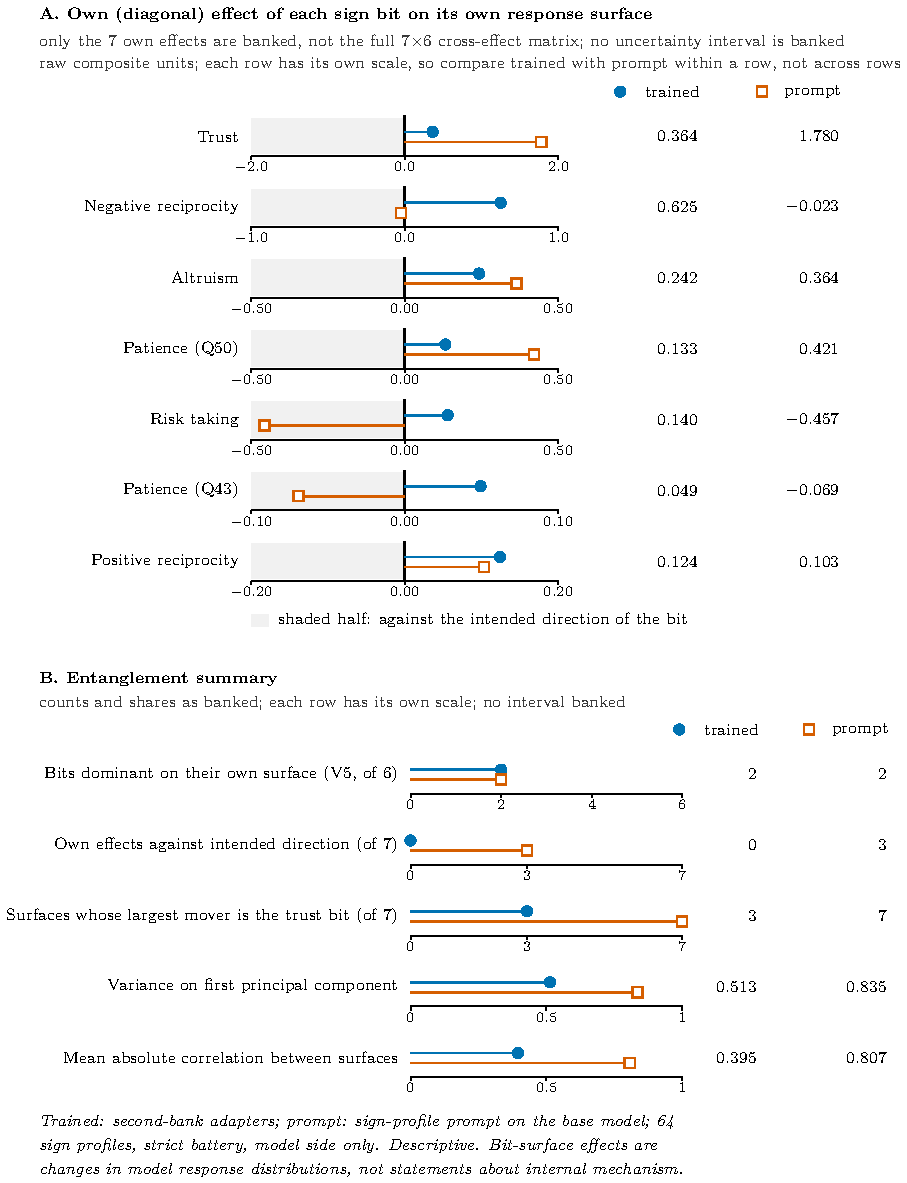
\includegraphics[width=0.91\textwidth]{figures/fig_factorial_own.pdf}
\caption{Own effects of the sign bits in the sixty-four-profile factorial (surface F; model side only). (A) For each of seven strict-battery surfaces, the main effect of the surface's own sign bit, for the trained second-cohort adapters (circles) and the sign-profile prompt (squares). All \cl{7}{FX_adapter64_own_effects_wrong_signed:n} trained own point estimates have the intended sign, and \cl{3}{FX_signprompt64_own_effects_wrong_signed} prompted ones do not. (B) Counts and shares that summarize entanglement. V5 was a planned check; the other rows are exploratory.}\label{fig:factorial}
\end{figure}

We next ask why the trust order survives when the other surfaces lose theirs. We split the second-cohort adapters' main effects into two parts: the effect of each surface's own bit and the summed effect of the other five. We evaluate each part at the sign profile of each of the \dc{42}{countries} countries and correlate it with the GPS coordinate of the surface's own dimension (D; the online supplement gives every surface). This is a behavioral decomposition that uses model quantities and published GPS values only. It says nothing about what happens inside the network. The own-bit part orders the countries like the GPS on all seven surfaces, with correlations from \cl{0.817}{C9_W1_patience_Q43_spearman_own_vs_gps} to \cl{0.866}{C9_W1_posrecip_spearman_own_vs_gps}. That ordering is mechanical. For a positive own effect, as all seven are, the own part is proportional to the sign of the GPS coordinate. It therefore restates the correlation between signs and GPS and is no separate test of learning. The full prediction, which adds the cross bits, keeps the GPS order on trust at \cl{0.834}{C9_W1_trust_spearman_full_vs_gps} and loses most of it elsewhere. On the other surfaces its correlations run from \cl{-0.020}{C9_W1_patience_Q43_spearman_full_vs_gps} for patience Q43 to \cl{0.422}{C9_W1_altruism_spearman_full_vs_gps} for altruism. The cross part carries little of the full prediction's variation on trust and most of it elsewhere. Var(cross)/Var(full) is \cl{0.147}{C9_W1_trust_cross_var_share} on trust and runs from \cl{0.830}{C9_W1_negrecip_cross_var_share} to \cl{1.049}{C9_W1_patience_Q43_cross_var_share} on the other six. This is a ratio of variances and no percentage of variance explained. It exceeds one on patience Q43 because the own and cross parts covary negatively. The comparison sets trust against six surfaces, so it is no graded relation and we claim no dose--response. No bank label depends on a second dimension. In both banks all \cl{27{,}636}{C9_W1_bank1_label_rows_checked} country-pair training rows follow the sign of the pair's own dimension, with \cl{0}{C9_W1_bank1_label_mismatches} mismatches in the first bank and \cl{0}{C9_W1_bank2_label_mismatches} in the second. Therefore, the labels do not carry the cross talk. We claim no cause of the loss, which would need component-level analysis and interventions.

Retraining noise is small beside these effects: an unseeded retrain of one profile moves every strict surface by at most \cl{0.112}{RP_max_abs_surface_diff_sd} of a standard deviation across profiles (R; online supplement). This is a narrow observed comparison of one retrained unit with its original. We did not measure variation across units.\footnote{The near-zero filter (N) is not promoted under the predeclared rule, and two refits support no claim of a reversal across countries. The online supplement gives the margin in full.}

\subsection{Instrument to respondents: the retrospective screen}\label{sec:res-screen}

Retrospectively, the screen rejects its registered null (H). The probe selected \cl{56}{SCR_A_primary:n} of the \dc{223}{pool_items} pool items under the primary rule. Their mean signed agreement with the Wave~7 country differences is $A=\cl{0.061}{SCR_A_primary}$ (Figure~\ref{fig:screen}, panel A), with a country-bootstrap interval of \ci{-0.007}{0.126}{SCR_A_primary}. The permutation null reassigns the same dimension and sign pairs to items drawn at random from the pool. Its distribution has mean \cl{0.012}{SCR_null_mean} and ninety-fifth percentile \cl{0.046}{SCR_null_q95}, and the one-sided $p$ is \cl{0.010}{SCR_p_perm} (panel B).

By the registered reading, the signal is weak. Two WVS waves agree with each other on the selected items fielded in both waves with a mean Spearman correlation of \cl{0.746}{SCR_ceiling_mean} (median \cl{0.767}{SCR_ceiling_median}, \cl{34}{SCR_ceiling_mean:n} items). The screen's $A$ is \cl{8.1}{SCR_A_over_ceiling:pct}\% of that ceiling, well below the registered bar of one third, which would be \cl{0.249}{SCR_one_third_ceiling}. The interval reaches zero while the permutation test rejects the null, because the two answer different questions. The test asks whether the assignments beat random assignments of the same pairs to items from the same pool. The interval asks how much $A$ varies across samples of countries. The direction of the finding is clearer than its size. The registered reliability checks point the same way. The secondary rule gives $A=\cl{0.070}{SCR_secondary_A}$ over \cl{185}{SCR_secondary_A:n} items with a one-sided permutation $p\cl{<0.001}{SCR_secondary_p_perm}$, and dropping one country at a time moves the primary $A$ only between \cl{0.051}{SCR_loco_min} and \cl{0.072}{SCR_loco_max}.

\begin{figure}[p]
\centering
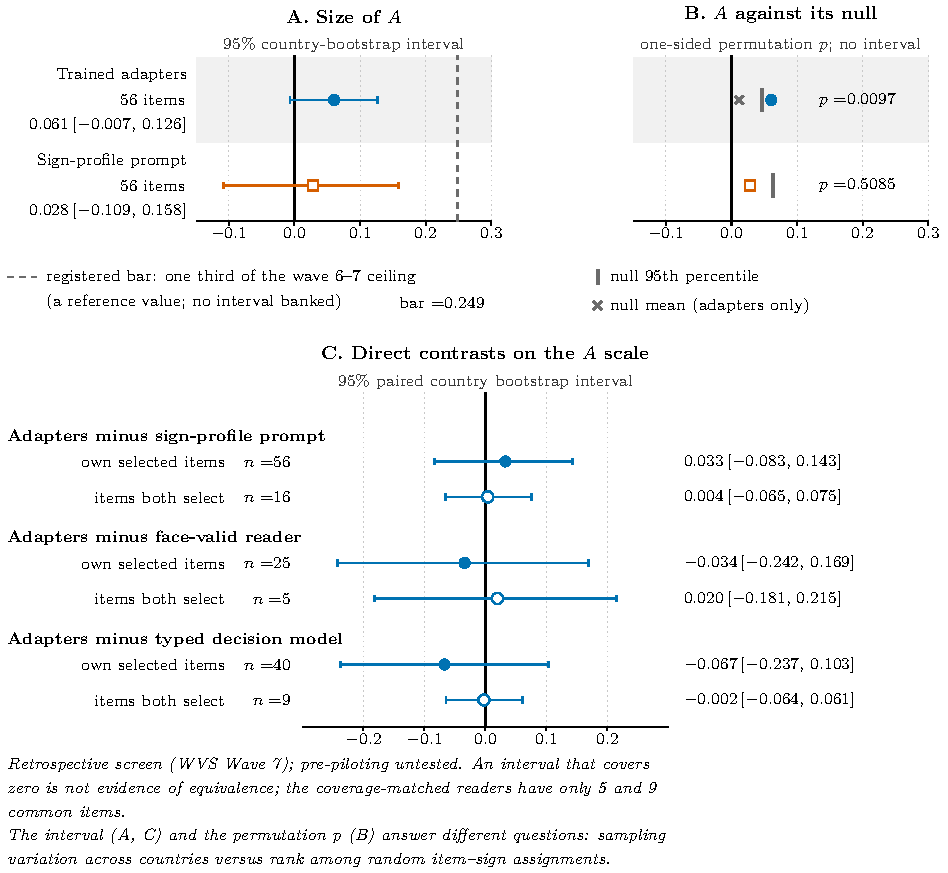
\includegraphics[width=\textwidth]{figures/fig_screen.pdf}
\caption{The retrospective held-out screen (surface H; preregistered, retrospective criterion). $A$ is the mean signed agreement, over the selected items, between the direction the probe assigned to an item and the WVS Wave~7 country differences on that item. (A) $A$ for the \cl{56}{SCR_A_primary:n} items the adapters selected and for the sign-profile prompt's own selection, with \dc{95}{ci_level}\% country-bootstrap intervals over \dc{42}{countries} countries; the dashed line is the registered bar of one third of the two-wave human ceiling, a reference value with no interval. (B) The same $A$ against its permutation null: the bar is the null's ninety-fifth percentile, the cross its mean (adapters only; none is banked for the prompt), and the one-sided $p$ is printed. (C) Paired contrasts, adapters minus each comparator, on each route's own items and on items both select ($n$ printed), with \dc{95}{ci_level}\% paired country-bootstrap intervals; the registered primary contrasts are those with questionnaire readers on shared items. Interval and permutation $p$ answer different questions, and an interval covering zero is not evidence of equivalence.}\label{fig:screen}
\end{figure}

The per-dimension readings show where the signal sits (Table~\ref{tab:checks}). Under the primary rule, only the items assigned to risk taking have an interval above zero. Their $A_d=\cl{0.158}{PD_adapter_primary_risktaking_A}$ \ci{0.015}{0.290}{PD_adapter_primary_risktaking_A} on \cl{13}{PD_adapter_primary_risktaking_A:n} items, of which \cl{92.3}{PD_adapter_primary_risktaking_share_pos:pct}\% agree in sign. The intervals for trust and altruism include zero. The items assigned to positive reciprocity point the wrong way: their point estimate is negative, and only \cl{18.2}{PD_adapter_primary_posrecip_share_pos:pct}\% of the \cl{11}{PD_adapter_primary_posrecip_share_pos:n} items agree in sign. Under the exploratory Bonferroni adjustment for four dimensions, the interval for risk taking becomes \ci{-0.026}{0.326}{PD_adapter_primary_risktaking_A_bonf} and includes zero.\footnote{The probe's per-dimension permutation $p$ values were not registered. For altruism under the primary rule they point the other way from the registered interval, so we report the registered intervals only.}

% Table 2: both checks per imprint dimension. Every number is a \cl / \ci macro tied to NUMBERS_TABLE.csv.
\begin{table}[htbp]
\centering
\caption{The second-bank check and the retrospective screen, by imprint dimension. The two checks are reported side by side and never averaged.}\label{tab:checks}
\small
\renewcommand{\arraystretch}{1.2}
\begin{tabularx}{\textwidth}{@{}>{\raggedright\arraybackslash}p{0.17\textwidth}>{\raggedright\arraybackslash}X>{\raggedright\arraybackslash}X>{\raggedright\arraybackslash}X>{\raggedright\arraybackslash}X@{}}
\toprule
 & S2: second bank & H: primary rule & H: primary rule, Bonferroni & H: secondary rule \\
Dimension & $\rho$ [\dc{95}{ci_level}\% interval] & $A_d$ [\dc{95}{ci_level}\% interval], items & $A_d$ [adjusted interval] & $A_d$ [\dc{95}{ci_level}\% interval], items \\
\midrule
Trust & \cl{0.803}{B2_bank2_trust_rho} \newline \ci{0.615}{0.876}{B2_bank2_trust_rho}
 & \cl{0.062}{PD_adapter_primary_trust_A} \newline \ci{-0.047}{0.173}{PD_adapter_primary_trust_A}, \cl{12}{PD_adapter_primary_trust_A:n}
 & \ci{-0.088}{0.199}{PD_adapter_primary_trust_A_bonf}
 & \cl{0.092}{PD_adapter_secondary_trust_A} \newline \ci{-0.019}{0.199}{PD_adapter_secondary_trust_A}, \cl{44}{PD_adapter_secondary_trust_A:n} \\
Risk taking & \cl{0.210}{B2_bank2_risktaking_rho} \newline \ci{-0.199}{0.584}{B2_bank2_risktaking_rho}
 & \cl{0.158}{PD_adapter_primary_risktaking_A} \newline \ci{0.015}{0.290}{PD_adapter_primary_risktaking_A}, \cl{13}{PD_adapter_primary_risktaking_A:n}
 & \ci{-0.026}{0.326}{PD_adapter_primary_risktaking_A_bonf}
 & \cl{0.143}{PD_adapter_secondary_risktaking_A} \newline \ci{0.045}{0.229}{PD_adapter_secondary_risktaking_A}, \cl{50}{PD_adapter_secondary_risktaking_A:n} \\
Positive reciprocity & \cl{0.366}{B2_bank2_posrecip_rho} \newline \ci{-0.068}{0.652}{B2_bank2_posrecip_rho}
 & \cl{-0.071}{PD_adapter_primary_posrecip_A} \newline \ci{-0.281}{0.154}{PD_adapter_primary_posrecip_A}, \cl{11}{PD_adapter_primary_posrecip_A:n}
 & \ci{-0.332}{0.205}{PD_adapter_primary_posrecip_A_bonf}
 & \cl{-0.049}{PD_adapter_secondary_posrecip_A} \newline \ci{-0.198}{0.117}{PD_adapter_secondary_posrecip_A}, \cl{22}{PD_adapter_secondary_posrecip_A:n} \\
Altruism & \cl{0.364}{B2_bank2_altruism_rho} \newline \ci{-0.057}{0.653}{B2_bank2_altruism_rho}
 & \cl{0.069}{PD_adapter_primary_altruism_A} \newline \ci{-0.036}{0.177}{PD_adapter_primary_altruism_A}, \cl{20}{PD_adapter_primary_altruism_A:n}
 & \ci{-0.058}{0.198}{PD_adapter_primary_altruism_A_bonf}
 & \cl{0.040}{PD_adapter_secondary_altruism_A} \newline \ci{-0.038}{0.117}{PD_adapter_secondary_altruism_A}, \cl{69}{PD_adapter_secondary_altruism_A:n} \\
\bottomrule
\end{tabularx}
\par\smallskip
\begin{minipage}{\textwidth}\footnotesize
\textit{Note:} S2 is the Spearman correlation between second-bank adapter composites and the GPS coordinate over \dc{42}{countries} countries, with a profile-block bootstrap (\dc{2,000}{boot_draws} draws, seed \dc{20261011}{seed_c3}); model side only. H is the retrospective screen against WVS Wave~7 country means: $A_d$ is the mean signed item agreement over the selected items assigned to the dimension, with the registered country bootstrap (\dc{2,000}{boot_draws} resamples, seed \dc{20261015}{seed_screen}). The registered intervals are unadjusted; the Bonferroni intervals over the \dc{4}{imprint_dims} imprint dimensions are exploratory and read off the same draws. The secondary rule is a registered reliability check. No dimension has an interval above zero on both S2 and H.
\end{minipage}
\end{table}


The two checks disagree by dimension. Trust survives the second bank, and its screen interval includes zero. Risk taking is the one dimension whose screen interval excludes zero before adjustment, and it is one of the three that lose their interval on the second bank. No dimension passes both registered checks, and the per-dimension cells are small.

\subsection{Instrument to respondents: questionnaire readers and the prompt route}\label{sec:res-comparators}

The registered contrasts do not distinguish the adapters from a careful reader of the questionnaire (Figure~\ref{fig:screen}, panel C; the online supplement tabulates every contrast). Every interval covers zero, which the preregistration reads as ``the adapters match a careful reader''. That reading rests on few items. The coverage-matched contrasts use the \cl{5}{CMP_face_valid_D_common:n} items that the adapters and the face-valid rule both assign and the \cl{9}{CMP_jev_D_common:n} items they share with the typed decision model. The routes agree on dimension and sign for \cl{1}{CMP_face_valid_common_same_dim_sign} and \cl{7}{CMP_jev_common_same_dim_sign} of them. An interval that covers zero on so few items is consistent with a match and does not establish one. Both readers concentrate on trust, where their own-item $A$ exceeds the \cl{0.062}{PD_adapter_primary_trust_A} of the adapters' own trust items, but their per-dimension cells are too small to be informative.

Prompting the base model with the same six signs does not pass the registered null. The same probe applied to the \dc{64}{cells} prompted profiles gives $A=\cl{0.028}{SP_A_primary}$ \ci{-0.109}{0.158}{SP_A_primary} with a one-sided permutation $p$ of \cl{0.509}{SP_p_perm}, and it assigns its selected items to a single dimension, trust. The adapter route passes the null and the prompt route does not, but the direct difference between them is unresolved. Adapter minus prompt is \cl{0.033}{SP_D_own} on each route's own items and \cl{0.004}{SP_D_common} on the \cl{16}{SP_overlap_with_adapter} items both select, and both intervals cover zero. The two routes agree on dimension and sign for \cl{6}{SP_overlap_same_dim_sign} of those shared items. We therefore cannot credit the trained weights over the prompt on the screen.

Item-level assignment is stable under option order and paraphrase, whereas membership in the particular selected set churns. The registered statistic is the number of selected items whose dimension and sign are unchanged. It is \cl{39}{RO_heldout_reverse_ds_unchanged} of \cl{56}{RO_heldout_reverse_ds_unchanged:n} with reversed options, \cl{39}{RO_heldout_para_a_ds_unchanged} with the first paraphrase and \cl{30}{RO_heldout_para_b_ds_unchanged} with the second. No variant changes more than half, so the registered condition for wording dependence is not met, although the second paraphrase comes close. Membership is another matter: the primary rule is a top-quartile cut on $|t|$, and only \cl{18}{RO_heldout_reverse_membership_agreement}, \cl{29}{RO_heldout_para_a_membership_agreement} and \cl{16}{RO_heldout_para_b_membership_agreement} of the \cl{56}{RO_heldout_para_b_membership_agreement:n} items are selected under both the original readout and each variant. Dimension and direction are more stable than the list of top-ranked items.

\subsection{Instrument to respondents: agreement with the human composite}\label{sec:res-human}

The next two subsections report descriptive follow-up analyses (D), added after the registered results had been read. None is preregistered and none enters a registered family. They set the instrument beside the respondents of the Wave~7 file on the strict battery, and every statement is retrospective. Figure~\ref{fig:links} gives three Spearman correlations over the \dc{42}{countries} countries for each of seven surfaces. They pair the adapter composite with the GPS, the adapter composite with the human composite of the same items, and the human composite with the GPS. The panels have different statistical targets and bootstrap units, so their widths are not comparable.

\begin{figure}[p]
\centering
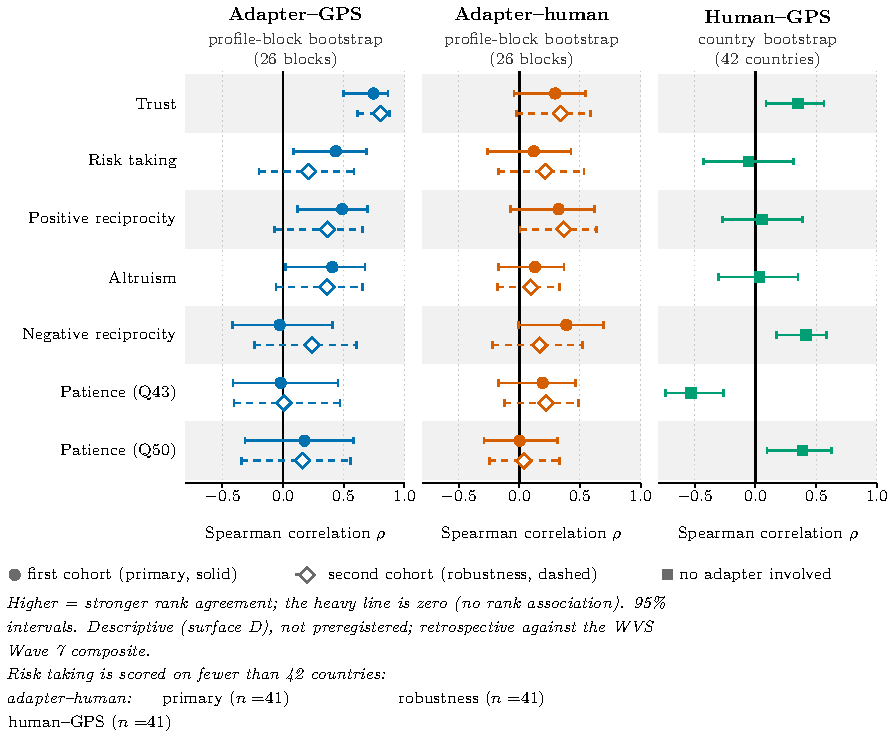
\includegraphics[width=\textwidth]{figures/fig_three_links.pdf}
\caption{The three links on seven strict-battery surfaces (surface D; descriptive, not preregistered; retrospective). Each mark is a Spearman correlation across countries with a \dc{95}{ci_level}\% interval; the heavy line is zero. Left: first-cohort adapter composite with the GPS coordinate of the surface's own dimension. Middle: adapter composite with the Wave~7 composite of the same items. Right: that human composite with the GPS. Circles are first-cohort adapters (primary), diamonds second-cohort adapters (robustness), squares involve no adapter. Intervals in the adapter panels come from a bootstrap over the \dc{26}{profiles_realized} realized sign profiles, those in the right panel from a bootstrap over the \dc{42}{countries} countries. Risk taking covers \cl{41}{C9_a_adapter_human_risktaking_spearman_rho:n} countries in the two human columns.}\label{fig:links}
\end{figure}

On trust, the first-cohort adapters track the GPS at \cl{0.744}{C9_a_adapter_gps_trust_spearman_rho} \ci{0.500}{0.865}{C9_a_adapter_gps_trust_spearman_rho}. They do not detectably reach the human composite, at \cl{0.295}{C9_a_adapter_human_trust_spearman_rho} \ci{-0.044}{0.547}{C9_a_adapter_human_trust_spearman_rho}. All seven adapter--human intervals include zero, which is not evidence that no association exists. The largest point estimate belongs to negative reciprocity, \cl{0.389}{C9_a_adapter_human_negrecip_spearman_rho} \ci{-0.008}{0.694}{C9_a_adapter_human_negrecip_spearman_rho}, a surface on which the adapters do not track the GPS. The second-cohort adapters give the same picture on trust, with an adapter--human correlation of \cl{0.340}{C9_b_adapter_human_trust_spearman_rho} \ci{-0.025}{0.586}{C9_b_adapter_human_trust_spearman_rho}. Positive reciprocity is the one second-cohort interval that excludes zero, and only just (online supplement).

The link between the GPS and the human composite is itself loose on these items. Its interval excludes zero on four of the seven surfaces. Among them, it is positive for trust at \cl{0.351}{C9_a_human_gps_trust_spearman_rho} \ci{0.088}{0.564}{C9_a_human_gps_trust_spearman_rho} and negative for patience Q43 at \cl{-0.533}{C9_a_human_gps_patience_q43_spearman_rho} \ci{-0.741}{-0.266}{C9_a_human_gps_patience_q43_spearman_rho}. We read this column as a reference for scale. It is no upper bound on what an adapter could reach, because it does not bound a scorer that is nonlinear or constant within sign profiles. Nor is it evidence that the anchor limits the instrument. Together, the three panels say that the adapters carry the GPS order on trust and that the GPS order is only loosely related to the human composite. They also show that the adapters' order of countries does not detectably agree with the human composite on any surface. The exact values for every cell are in the online supplement.

\subsection{Instrument to respondents: order versus distance}\label{sec:res-tvd}

The correlations above concern the order of countries. A different question is how far the instrument's response distribution lies from the survey's. We measure it by the country-equal mean total variation distance (TVD; lower is closer; D) in four cells. They are the base model and the first-cohort adapters, each with and without the country-named persona prompt.

The base model's mean distance is \cl{0.470}{C9_TVD_base_mean_tvd_country_equal}. The adapters sit farther from the survey at \cl{0.515}{C9_TVD_adapter_mean_tvd_country_equal}, and the persona prompt sits closer at \cl{0.365}{C9_TVD_persona_mean_tvd_country_equal} (panel B of Figure~\ref{fig:route}). A cell mean carries no interval, whereas the paired contrasts of panel C each carry one. Relative to the base model, the adapters are farther by \cl{0.045}{C9_TVD_adapter_minus_base_profile_block} \ci{0.006}{0.093}{C9_TVD_adapter_minus_base_profile_block} under profile blocks, and the persona prompt is closer by \cl{-0.105}{C9_TVD_persona_minus_base_profile_block} \ci{-0.122}{-0.086}{C9_TVD_persona_minus_base_profile_block}. Country resampling gives the same readings. With both interventions the distance is \cl{0.420}{C9_TVD_adapter_persona_mean_tvd_country_equal}. Adding the persona prompt to the adapters moves the distance by \cl{-0.096}{C9_TVD_adapter_persona_minus_adapter_profile_block} \ci{-0.115}{-0.078}{C9_TVD_adapter_persona_minus_adapter_profile_block}, and adding the adapters to the persona prompt moves it by \cl{0.055}{C9_TVD_adapter_persona_minus_persona_profile_block} \ci{0.016}{0.097}{C9_TVD_adapter_persona_minus_persona_profile_block}. The interaction contrast is the adapters' effect with the persona prompt minus their effect without it. Under profile blocks it is \cl{0.009}{C9_TVD_interaction_profile_block} \ci{-0.003}{0.022}{C9_TVD_interaction_profile_block}, an interval that includes zero. Therefore, the data show no detectable departure from additivity.

\begin{figure}[p]
\centering
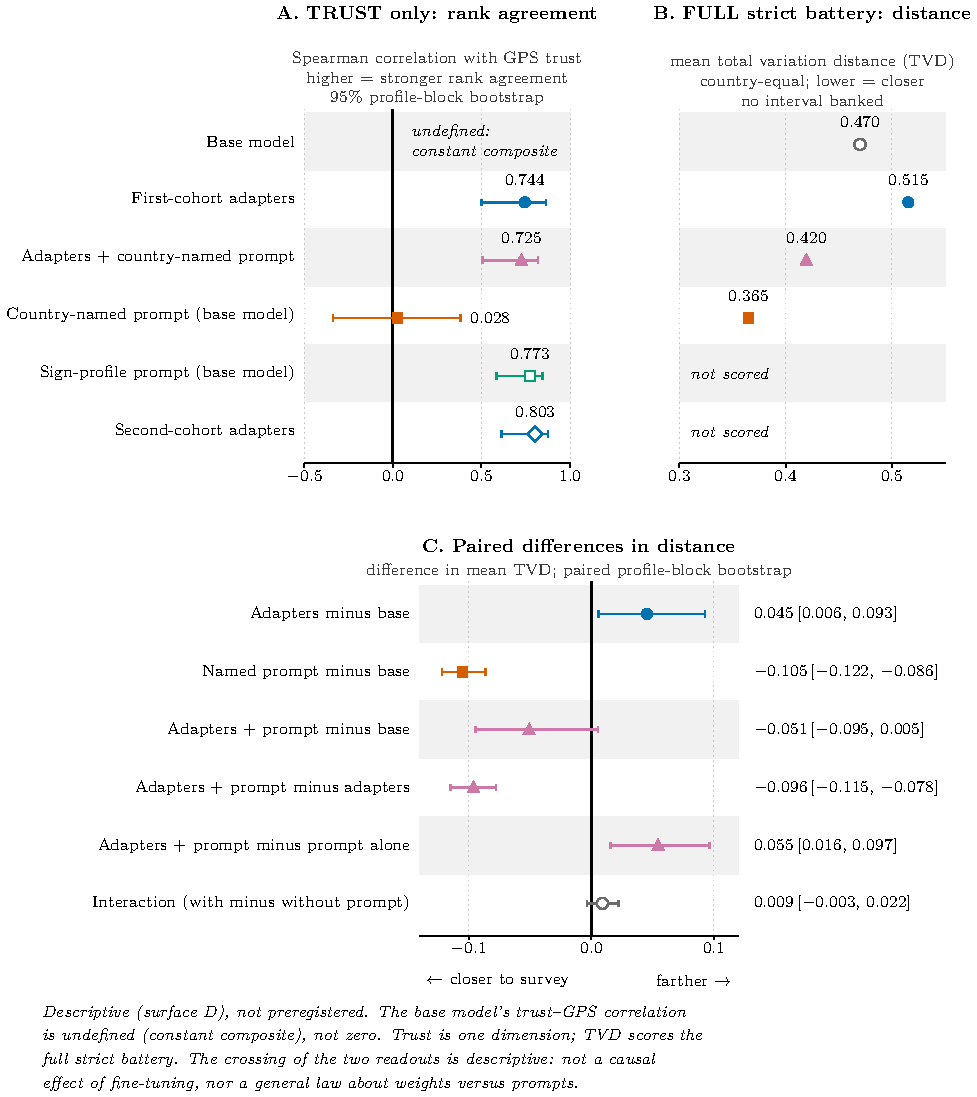
\includegraphics[width=0.98\textwidth]{figures/fig_info_vs_route.pdf}
\caption{Order and distance for the same routes (a descriptive display, not preregistered; the distances are retrospective). (A) Trust only: Spearman correlation of each route's trust composite with the GPS trust coordinate over \dc{42}{countries} countries, with \dc{95}{ci_level}\% profile-block intervals. The first-cohort, second-bank and country-named values are those of Section~\ref{sec:res-bank}, where their own status is stated. (B) Mean total variation distance (TVD) to the survey answer shares over the full strict battery, country-equal; routes not scored on this battery are marked. (C) Paired differences in mean TVD with \dc{95}{ci_level}\% profile-block intervals; negative means the first-named cell is closer. Panel A scores trust only and panels B and C all dimensions, so they are different metrics.}\label{fig:route}
\end{figure}

The ordering of the cells by distance does not follow their ordering by trust agreement with the GPS. The persona prompt has the lowest distance and no trust order (Section~\ref{sec:res-bank}). The adapters have the highest distance and keep the trust order. Adding the persona prompt to the adapters keeps the trust order at \cl{0.725}{C9_TVD_adapter_persona_trust_gps_profile_block} \ci{0.505}{0.820}{C9_TVD_adapter_persona_trust_gps_profile_block} while the distance falls.

\section{Discussion}\label{sec:discussion}

We asked a language model only about the group, and the answer comes in two parts that point in opposite directions. Conditioned on declared group signs, the instrument keeps the GPS order of countries on trust, also on a second scenario bank. Checked against the Wave~7 respondents, its order of countries does not detectably agree with theirs, and its response distributions sit farther from theirs than the base model's do. In other words, it can order countries the way a cross-national survey does while answering unlike the people in them.

\paragraph{The conditioning method: what the signs carry.} The declared sign carries the trust order, whichever channel supplies it. The adapters keep the trust order across scenario banks (Section~\ref{sec:res-bank}). A country name does not recover that order, whereas a prompt that states the six signs does. On trust the sign prompt correlates with the GPS at \cl{0.773}{PX_signprompt_trust_rho} \ci{0.584}{0.844}{PX_signprompt_trust_rho}, against \cl{0.028}{PX_persona_trust_rho} \ci{-0.339}{0.381}{PX_persona_trust_rho} for the named country. In the screen, we could not resolve the contrast between the adapters and the sign prompt. Therefore, the evidence cannot credit the trained weights over a prompt, and the statement concerns trust only. The decomposition of the factorial shows where trust differs from the other surfaces. Every own effect is positive, so the own part of the main-effects prediction restates the correlation between the signs and the GPS on every surface. What differs is how much the other five signs add. On trust they add little, with Var(cross)/Var(full) at \cl{0.147}{C9_W1_trust_cross_var_share}. On the other six surfaces they carry most of the variation, with ratios from \cl{0.830}{C9_W1_negrecip_cross_var_share} to \cl{1.049}{C9_W1_patience_Q43_cross_var_share}. The decomposition describes behavior and leaves open why the other dimensions lose their order.

Training on sign-labeled pairs keeps the direction of each declared input and does not deliver separate dimensions. Each sign moves its own surface in the intended direction and also moves other surfaces. One common direction carries about half of the variance across surfaces, and the planned separability check fails on both routes. Prompting with the same signs is more entangled still, and three of its own effects point the wrong way. Entanglement under intervention has also been reported when cultural values are edited through a model's internal activations \citep{dangmasud2026}. Our factorial adds a joint measurement for trained adapters and for a prompt that carry the same declared information. We make no claim about the best training recipe.

\paragraph{The evaluation protocol: what it separates.} Each part of the protocol separated something that a single agreement figure would have merged. Notably, separating the three links showed that the GPS's own agreement with the human composite is loose on these items. Weak adapter--human agreement therefore cannot be attributed to the instrument alone. It could arise from the instrument, from the mapping between items and the GPS construct, or from limited coherence between the two surveys. The design cannot tell these apart. The registered screen and its freeze sequence are fixed before the human criterion is read, and we label the descriptive analyses added afterwards as such. Another team can therefore apply the protocol to a different conditioning method, anchor or criterion.

\paragraph{Order and distribution.} The split between order and distribution is what a group-level design gives us reason to expect. We chose to model the group directly and left the aggregation over people to the GPS. An order of countries needs only a score that rises with the group's latent preference, and no representative respondent whose answers equal the population's \citep{kirman1992}. A single choice policy per country, however, has no spread within the country built in. That is, it can carry an order and has no reason to match the distribution of respondents' answers. We offer one reading without testing it: the training signal states which of two responses is preferred and says nothing about how strongly, or about how widely respondents spread across the options. The order of countries is a quantity that signs speak to, whereas a distance to the survey's response distributions is one they carry no information about. This argument explains why the adapters have no reason to approach the survey's response distributions. It does not explain why they move away from them, or why a country-named prompt moves toward them.

The evidence shows the two targets crossing (Section~\ref{sec:res-tvd}). The adapters keep the anchor's order of countries on trust and lie farther from the survey's response distributions than the base model, by \cl{0.045}{C9_TVD_adapter_minus_base_profile_block} \ci{0.006}{0.093}{C9_TVD_adapter_minus_base_profile_block} in total variation distance. A country-named prompt lies closer, by \cl{-0.105}{C9_TVD_persona_minus_base_profile_block} \ci{-0.122}{-0.086}{C9_TVD_persona_minus_base_profile_block}, and carries no trust order. If agreement were one quantity, the routes would fall in one ranking. They fall in two. The contrast describes one anchor, one instrument family and one survey, and it does not show that the country-named prompt matches respondents. A country name has been found to recover a country ranking in the European Social Survey while supporting no distributional inference \citep{wangc2026}. The separation of group-level order from distributional fidelity is established \citep{dasilva2026}. Our case adds one method whose two answers point in opposite directions, so order and distribution have to be validated separately.

\paragraph{What a prospective validation would have to establish.} A prospective validation would have to establish three things that the retrospective design cannot. First, the probe's selections and a human-only rule for choosing items would both be declared before any new items are fielded. Second, the selected items would have to separate countries in the assigned direction in new data. They would also have to do so better than the human-only rule on matched countries and items. Third, the dimension on which the signal appears would have to be one that the second bank also supports. We would read a result of that kind as licensing the use before fielding. Whether such a test would find the signal on trust, the one dimension the second bank supports, is the open question this paper leaves.

\paragraph{Limits.} Five limits apply to every result above. First, the human criterion is retrospective and is the only human source. Registration and the freeze guard protect against tuning the probe to it. They cannot make it independent of the survey program from which the item pool was drawn. Second, we chose the country as the unit, and our claims stay at that unit. The instrument is built from signs and cannot represent magnitudes, differences among countries that share a sign profile, or variation among people within a country. Country-level agreement does not establish individual-level validity or measurement invariance \citep{davidov2014,bratt2025}. Third, all our adapters share one base model, one training recipe and one readout convention. Their code probabilities have a dispersion that need not match human response distributions. Fourth, the per-dimension cells are small and the selected set churns under readout variants. Fifth, the noise checks are narrow. One unseeded retrain is a narrow observed comparison for one unit, and two near-zero refits support no claim across countries.

\paragraph{Intended use.} Within those limits, the instrument has a modest and inspectable use. A survey designer can read the dimension and direction it assigns to candidate items as one input beside expert review and human pretesting, keeping in view that no dimension passed both checks. We see it as a complement to fielding and pretesting, and the evidence gives no reason to replace them. In the terms of \citet{broska2025}, its readings are potentially informative observations that still require a human criterion.

\section{Conclusion}\label{sec:conclusion}

Preserving an external benchmark is evidence about the link between benchmark and method. For synthetic cultural agents, which compile declared aggregate preference signs into choice policies that read survey items without naming a group, we tested each link of the chain from anchor to instrument to respondents separately.

Between anchor and instrument the method holds in a limited sense. Training installs the synthetic labels on pairs the adapters never saw, and on trust the adapters keep the anchor's order of countries across a change of scenario bank. A country name does not keep that order, and a prompt stating the same signs does, so the declared signs carry the trust order and the evidence cannot credit the trained weights over a prompt. The adapters do not keep the declared dimensions separate. Between instrument and respondents the evidence is weak. A preregistered screen of held-out items, read against a retrospective criterion, gives a small signal that the registered comparisons do not separate from careful readers of the questionnaire, no dimension passes both the second-bank check and the screen, and the adapters' order of countries does not detectably agree with the respondents' composite. Keeping the anchor's order of countries and approaching respondents' answer distributions are different questions, and on a descriptive reading the adapters keep the first and lie farther from the survey's answer distributions than the base model, whereas a country-named prompt lies closer with no trust order.

The method is an inspectable, group-level reading of candidate items that a researcher may use beside human pretesting, as a complement and never in its place. The evaluation protocol applies to other conditioning methods and other anchors. The test that would license more is prospective: probe-selected items fielded to people after the selection and a human-only comparison rule have both been declared. Until that test is run, pre-piloting remains untested.

% Backmatter in SMR order (venue card): preregistration; code, materials and data availability; institutional
% review; conflicting interests; funding; generative AI. Acknowledgements are on title_page.tex (anonymized review).
\section*{Preregistration Statement}

The held-out screen (Sections~\ref{sec:design-screen} and \ref{sec:res-screen}) was preregistered. The registration document was committed to the project repository and timestamped by the git tag \texttt{prereg-heldout-2026-10-14}, pushed before any held-out item was scored by an adapter. Amendment~1 (repair of \dc{12}{repaired_items} items whose standalone wording could not be answered) was made after the first model-side probe pass had been computed and read, and before any human value was read. The freeze file was committed, and Amendment~2 (removal of those items from both comparator routes) was decided, before the single read of held-out human data; the text of Amendment~2 was written afterwards and records that earlier decision. The criterion data, WVS Wave~7, are public and existed before the study, so the registration fixes the analysis before the authors read the human values and the criterion remains retrospective. All registered analyses of the screen are reported in Section~\ref{sec:res-screen}, Table~\ref{tab:checks} and Figure~\ref{fig:screen}, except two descriptives (item-level agreement after dropping items with small $|a_i|$, and the face-valid reader's statistic on all of its items including negative reciprocity), which are reported in the online supplement.
The Bonferroni intervals, the wave-specific screen statistics, the scale-free factorial views and the factorial route contrast are exploratory. The factorial's separability check (V5) was fixed in the project's analysis plan, separately from the registration. The second-bank decision rule was fixed before the second cohort was trained and was not part of the registration. An anonymized copy of the registration is provided with the submission. % TODO(Augusto): register the tagged document at an institutional registry (e.g., OSF). The registry copy will be dated after data access, and this statement must say so.

\section*{Code, Materials, and Data Availability}

Analysis code, the item pool and its overrides, the frozen selection, the comparator files, all model scores, and the scripts that build every number in this article from those scores are available for review at an anonymized link. % TODO(Augusto): anonymized mirror for review (e.g., anonymous.4open.science of the repository).
Model adapters and score archives are released at acceptance. The frozen inputs are identified by SHA-256 hashes: the amended item pool \clh{19241f6f103c51d6}{HASH_pool_worktree}\ldots{} as written to disk, whose line-ending-normalized form in the repository is \clh{a1dbceea1a33da05}{HASH_pool_git_blob_lf}\ldots{}; the overrides file \clh{0f5cd2bbd88ef6ea}{HASH_overrides}\ldots{}; and the frozen selection \clh{782b7d2123f9758e}{HASH_selection_amended_20261016}\ldots{}. The pool is regenerated byte for byte from the overrides file by the pool-building script; full hashes and the line-ending convention are in the online supplement. WVS and GPS data are available from their providers \citep{wvs2022,wvsts2022,falk2018} and are not redistributed; no respondent-level data or country-level human means are included in the replication materials.

\section*{Institutional Review}

This study analyzes publicly available, de-identified secondary survey data and involves no interaction with human participants. % TODO(Augusto): confirm the institutional review determination for secondary public data.

\section*{Declaration of Conflicting Interests}

The authors declared no potential conflicts of interest with respect to the research, authorship, and/or publication of this article. % TODO(Augusto): confirm for this paper (the confirmation on record covers the earlier preprint), including any relationship with the provider of the typed decision model used as a comparator.

\section*{Funding}

The authors received no financial support for the research, authorship, and/or publication of this article. % TODO(Augusto): confirm for this paper, including compute credits.

\section*{Declaration of Generative AI Use}

Large language models are the object of study in this article. In addition, an AI coding and writing assistant was used under the authors' direction to write analysis code and to draft and edit manuscript text; the authors reviewed all code, numbers and text and take responsibility for them. % TODO(Augusto): confirm wording and name the tools as SMR requires.

\singlespacing
\bibliographystyle{chicago}
\bibliography{references}
\end{document}
